% Technical report. Set from report/draft.md, which is committed beside this file
% so the input and the output move together and the translation is diffable.
%
% Build:  make -C report        (or: latexmk -pdf main.tex, from this directory)

\documentclass[11pt]{article}

% Standard margins, stated rather than defaulted, because the figures are sized
% against \textwidth. At letterpaper with 1 in margins \textwidth is exactly
% 6.5 in, which is the width report/figures/make_*.py draw to, so a figure
% included at width=\textwidth is reproduced 1:1 and its type is not rescaled.
\usepackage[letterpaper,margin=1in]{geometry}

\usepackage[T1]{fontenc}
\usepackage{lmodern}
\usepackage{graphicx}
\usepackage{booktabs}
\usepackage[hidelinks]{hyperref}

% biblatex + biber, not bibtex. biber was present when the choice was made and
% ships with the TeX Live installation CI uses, and biblatex is what carries the
% per-entry provenance notes this report's bibliography needs -- including a
% software entry pinned to a commit rather than to a branch.
\usepackage[backend=biber,style=numeric,sorting=none]{biblatex}
\addbibresource{refs.bib}

\graphicspath{{figures/}}

\title{Experiments on Active 3D Vision}

% Two authors. The collaborator footnote is draft.md's own, set here rather than
% in the body: it is a statement about authorship and belongs on the byline.
\author{
  Luiz Velho\\
  \normalsize IMPA
  \and
  Claude\thanks{This technical report was produced in collaboration with Claude
  --- model Opus, high reasoning effort. See Appendix~A for what each surface did
  and why authorship is attributed as it is.}\\
  \normalsize Anthropic (collaborator)
}

\date{\today}

\begin{document}
\maketitle

\begin{abstract}
Active vision holds that perception is better posed as a controlled sampling
problem than as a reconstruction problem: that choosing where to look improves
what is perceived. This report tests that claim for binocular depth estimation,
in a framework built on oculomotor geometry --- eyes rotating about fixed
centres, vergence setting the horopter, torsion determined by gaze --- and a
Bayesian belief accumulated across fixations.

Thirteen pre-registered experiments give a consistent negative answer to the
question as posed. The gaze objective did not matter; two objectives that never
once selected the same pixel produced indistinguishable results. On a stimulus
with effectively no occlusion, knowing \emph{where} measurement is possible
outweighed knowing \emph{how uncertain} it is by 65:1 on median error. Foveal
weighting on a uniformly sampled sensor was strictly lossy. Verging to acquire made estimation worse, through a mechanism
that generalises beyond stereo: a controller driven by a statistic over
\emph{valid} measurements is blind to the error that would correct it. Closing
the perception--action loop did help, at 41\texttimes{} the cost --- but the
benefit was coverage over accuracy by at least 33\texttimes{}. The system's
advantage was that it saw the scene, not that it estimated better.

Four of the thirteen experiments were about the instrument or the criterion
rather than about the framework, and were the precondition for reading the
rest. We conclude that the
framework may have posed a budget problem as an estimation problem: foveation in
a retina means \emph{not paying} for the periphery, and implemented as weighting
it can only discard information already bought. The complete record is public.
\end{abstract}

% Set from report/draft.md, part 1. The prose is the maintainer's; this file is
% its transit into LaTeX and nothing in it was rewritten.
\section{Introduction}

\subsection{Motivation: active vision as sampling under a budget}

Open a camera's shutter and every pixel arrives at the same resolution. Open an
eye and it does not. The human fovea subtends one to two degrees of high acuity;
beyond it resolution falls off sharply, and three or four times a second a
saccade repositions that window somewhere new. The retina is not a uniform
sensor that attention is later applied to. It is a variable-resolution sensor,
and foveation is a bandwidth decision before it is an attention mechanism.

That distinction is easy to state and, as this report will show, easy to lose in
implementation. It is the hinge on which most of what follows turns.

Binocular vision adds a second sense in which biological vision is \emph{active}.
The eyes are not two cameras with fixed extrinsics. They rotate about centres
fixed in the head; vergence sets the distance at which the two lines of sight
intersect; and the torsion of each eye is not free but determined by gaze
through Listing's law --- the eye's orientation lies in a plane that tilts with
vergence. Stereo geometry in a biological system is therefore \emph{oculomotor}:
it follows from where the system is looking, and it changes every time it looks
somewhere else.

This report describes a project that took that framing literally. The claim
under test is the one the active-perception tradition has advanced since the
1980s --- Bajcsy's \emph{Active Perception}~\cite{bajcsy1988active}, Aloimonos,
Weiss and Bandyopadhyay's \emph{Active Vision}~\cite{aloimonos1988active},
Ballard's \emph{Animate Vision}~\cite{ballard1991animate} --- that perception is
better posed as a controlled sampling problem than as a reconstruction problem.
Applied to stereo depth, the specific question becomes: does choosing where to
look improve depth estimation, relative to not choosing?

The stimulus deserves its own mention. Julesz's random-dot
stereograms~\cite{julesz1960binocular} isolate stereopsis by removing every
monocular depth cue --- depth exists only in disparity, so a system that appears
to recover it cannot be exploiting shading or texture gradient. That property
made them the natural synthetic fixture here. It also made a defect in that
fixture unusually damaging, in a way \S2 takes up.

\subsection{Background: stereo depth as inference}

Stereo matching admits a Bayesian reading. For each pixel, comparing a patch
against candidate positions in the other image produces a cost curve over
disparity --- a likelihood. A prior over depth or a smoothness assumption
supplies the rest, and the quantity of interest is the posterior: an estimate
with an uncertainty attached, not a point estimate.

Uncertainty is usually read from the cost curve. Curvature at the minimum gives
a local precision; the ratio between the best and second-best minima measures
ambiguity; agreement between left-to-right and right-to-left matching flags
pixels with no consistent correspondent. Estimates from multiple views are then
combined by precision weighting --- each measurement contributes in proportion
to its confidence.

Depth is not disparity. Recovering metric depth requires knowing the geometry,
and for a converged binocular system it requires knowing the fixation distance.
This is where the oculomotor framing enters the estimator rather than just the
camera model, and it is the origin of one of the report's more portable
findings.

One property of this pipeline must be stated, because it motivated the work and
because the record complicates it. A half-occluded pixel --- visible to one eye,
hidden from the other --- has no true correspondent. The matcher does not report
this; it finds the best available wrong match, and a sharp cost minimum at a
wrong disparity is genuinely sharp. The result is a confident, incorrect
estimate at exactly the geometry an active system might hope to resolve by
looking elsewhere.

The predecessor repositories measured this on photographs, across three
uncertainty readouts, and found variance in half-occluded regions \emph{lower}
than in matched ones --- confidence inverted where it matters most. On
random-dot stereograms the same matcher and the same statistic give the
opposite: variance roughly twice as high in half-occlusions, which is the safe
direction.

So the failure is not a stimulus-independent property of stereo confidence. It
appears on real imagery and not on synthetic dots, and whether that difference
is about realism or about contrast is unresolved --- a random-dot field is
contrast-uniform by construction and cannot separate them. That open question is
the sharper motivation: confidence fails where the scene is real, and the
synthetic fixture this project used sits on the safe side of the reversal.

\subsection{Concepts}

Four distinctions do most of the analytical work, and none was fully in place
when the project began.

\textbf{Allocation versus acquisition.} \emph{Where to spend limited processing
on data already sampled}, against \emph{where to point the sensor to obtain data
not yet sampled}. Most treatments of active vision conflate them. Separating
them is what makes the results here interpretable, and the separation has a
clean geometric form: a rotation about a fixed optical centre changes allocation
and cannot change acquisition.

\textbf{Unknowable is not uncertain.} A pixel with no valid correspondent is not
a pixel we are unsure about; it is one we cannot measure. The difference between
a binary \emph{can this be measured} and a continuous \emph{how well} turned out
to dominate.

\textbf{Foveal weighting versus foveal sampling.} Weighting says the fovea
contributes more to the posterior. Sampling says the periphery was never
resolved in the first place. On a uniformly sampled sensor the first can only
discard information already paid for. Only the second is what a retina does.

\textbf{Linearising about the fixation is a confidence mechanism.} Expanding the
depth relation about the fixated disparity is exact at the fovea and degrades
with the square of the offset. That degradation term does more than bound
approximation error: it inflates the variance of any estimate far from the
fixated depth, and thereby refuses precisely the confident-and-wrong matches
described above.

A fifth concept was not brought to the project but forced on it, and \S2 begins
there: a stimulus is an instrument, and must be characterised before it is used
to measure.

\subsection{Architecture}

\begin{figure}[htbp]
  \centering
  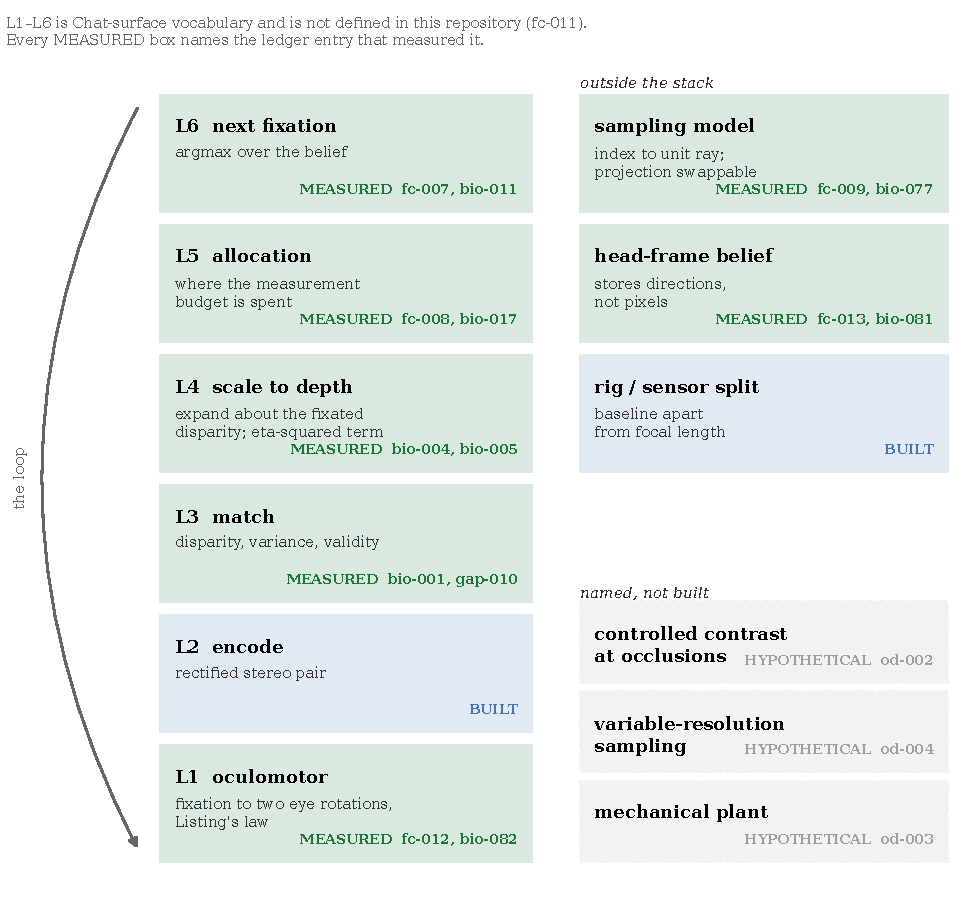
\includegraphics[width=\textwidth]{architecture.pdf}
  \caption{The six-layer framework, with the three components that sit outside
  it and the three that are named but not built. \emph{Measured} means the
  ledger contains a measurement of the layer's behaviour, and every such box
  names the foreclosure or measurement entry it rests on; \emph{built} means
  implemented and tested with no measurement bearing on the question the layer
  exists to answer; \emph{hypothetical} means recorded as an open decision and
  not built. Drawn from the structure of \texttt{docs/state.yaml} and
  \texttt{docs/inherited-measurements.yaml}, and the script asserts that every
  cited id exists in one of them before it draws. The layer numbering
  \texttt{L1}--\texttt{L6} is Chat-surface vocabulary and is not defined in the
  repository (\texttt{fc-011}).}
  \label{fig:architecture}
\end{figure}

The framework is six layers, and a pass through the loop is the clearest way to
describe them.

A fixation is a gaze direction and a vergence. \textbf{L1} turns it into two eye
rotations under Listing's law, which places the cameras. \textbf{L2} encodes the
resulting pair; \textbf{L3} matches, producing disparity with a variance and a
validity mask. \textbf{L4} scales disparity to metric depth by expanding about
the fixated disparity --- first-order-exact at the fovea, degrading as the
square of the offset. \textbf{L5} decides where attention is allocated;
\textbf{L6} picks the next fixation from the belief's uncertainty. The belief
updates, and the loop repeats.

The layers are not equally weighted in practice. L1 is substantial and was
expensive to get right; L2 and L3 are deliberately minimal; L4 carries more than
its size suggests, through the Jacobian that converts disparity variance into
depth variance; L5 was decided as attentional allocation with the mechanical
branch left untested; L6 is a two-line argmax that, as \S2.2 reports, turned out
not to matter.

Three components sit outside the six-layer stack, and each exists because the
stack alone was insufficient.

\textbf{The sampling model} maps a sample index to a unit ray. It is what makes
the projection swappable: a spherical sensor satisfied the same interface as a
pinhole one without a signature change, because the frame is identical and only
the index-to-direction map differs --- which is the whole of what a projection
is.

\textbf{The belief} is head-anchored and stores directions rather than pixels,
so it survives a change of projection untouched. Its failure mode was
instructive: tied initially to the rectifying rotation, which ignores azimuth by
construction, it silently fused measurements of different world directions into
the same cell, and no test caught it because every control varied elevation.

\textbf{The rig/sensor split.} The original rig type carried baseline and focal
length together, which coupled two thirds of the geometry tests to an intrinsic
they did not need. Separating stereo geometry from the sensor is what made the
rotational content portable.

Listing's tilt is a parameter, not a constant: the default is 0.25 per radian of
vergence, while 0.5 is the value at which vertical disparity in the plane of
regard vanishes exactly. The two are distinct and the distinction is pinned by
test.

% Set from report/draft.md section 2. The prose is the maintainer's; this file is
% its transit into LaTeX and nothing in it was rewritten.
\section{Background}

\subsection{Stereo depth as inference}

Stereo matching admits a Bayesian reading. For each pixel, comparing a patch
against candidate positions in the other image produces a cost curve over
disparity --- a likelihood. A prior over depth or a smoothness assumption
supplies the rest, and the quantity of interest is the posterior: an estimate
with an uncertainty attached, not a point estimate.

Uncertainty is usually read from the cost curve. Curvature at the minimum gives
a local precision; the ratio between the best and second-best minima measures
ambiguity; agreement between left-to-right and right-to-left matching flags
pixels with no consistent correspondent. Estimates from multiple views are then
combined by precision weighting --- each measurement contributes in proportion
to its confidence.

Depth is not disparity. Recovering metric depth requires knowing the geometry,
and for a converged binocular system it requires knowing the fixation distance.
This is where the oculomotor framing enters the estimator rather than just the
camera model, and it is the origin of one of the report's more portable
findings.

One property of this pipeline must be stated, because it motivated the work and
because the record complicates it. A half-occluded pixel --- visible to one eye,
hidden from the other --- has no true correspondent. The matcher does not report
this; it finds the best available wrong match, and a sharp cost minimum at a
wrong disparity is genuinely sharp. The result is a confident, incorrect
estimate at exactly the geometry an active system might hope to resolve by
looking elsewhere.

The predecessor repositories measured this on photographs, across three
uncertainty readouts, and found variance in half-occluded regions \emph{lower}
than in matched ones --- confidence inverted where it matters most. On
random-dot stereograms the same matcher and the same statistic give the
opposite: variance roughly twice as high in half-occlusions, which is the safe
direction.

So the failure is not a stimulus-independent property of stereo confidence. It
appears on real imagery and not on synthetic dots, and whether that difference
is about realism or about contrast is unresolved --- a random-dot field is
contrast-uniform by construction and cannot separate them. That open question is
the sharper motivation: confidence fails where the scene is real, and the
synthetic fixture this project used sits on the safe side of the reversal.

\subsection{Concepts}

Four distinctions do most of the analytical work, and none was fully in place
when the project began.

\textbf{Allocation versus acquisition.} \emph{Where to spend limited processing
on data already sampled}, against \emph{where to point the sensor to obtain data
not yet sampled}. Most treatments of active vision conflate them. Separating
them is what makes the results here interpretable, and the separation has a
clean geometric form: a rotation about a fixed optical centre changes allocation
and cannot change acquisition.

\textbf{Unknowable is not uncertain.} A pixel with no valid correspondent is not
a pixel we are unsure about; it is one we cannot measure. The difference between
a binary \emph{can this be measured} and a continuous \emph{how well} turned out
to dominate.

\textbf{Foveal weighting versus foveal sampling.} Weighting says the fovea
contributes more to the posterior. Sampling says the periphery was never
resolved in the first place. On a uniformly sampled sensor the first can only
discard information already paid for. Only the second is what a retina does.

\textbf{Linearising about the fixation is a confidence mechanism.} Expanding the
depth relation about the fixated disparity is exact at the fovea and degrades
with the square of the offset. That degradation term does more than bound
approximation error: it inflates the variance of any estimate far from the
fixated depth, and thereby refuses precisely the confident-and-wrong matches
described above.

A fifth concept was not brought to the project but forced on it, and \S3.3 takes
it up: a stimulus is an instrument, and must be characterised before it is used
to measure.

% Set from report/draft.md section 3. The prose is the maintainer's; this file is
% its transit into LaTeX and nothing in it was rewritten.
%
% Every caption states what was measured, on what, and cites the ledger entries
% the numbers come from.
\section{Overview}

\subsection{Architecture}

\begin{figure}[htbp]
  \centering
  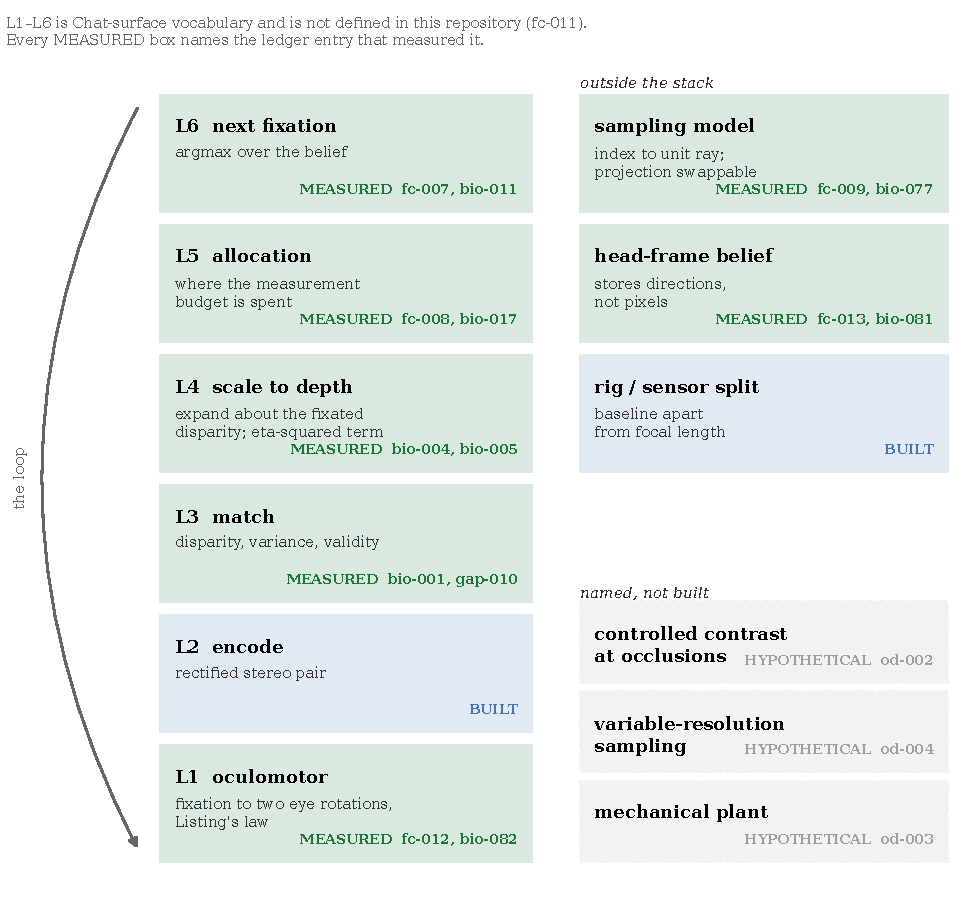
\includegraphics[width=\textwidth]{architecture.pdf}
  \caption{The six-layer framework, with the three components that sit outside
  it and the three that are named but not built. \emph{Measured} means the
  ledger contains a measurement of the layer's behaviour, and every such box
  names the foreclosure or measurement entry it rests on; \emph{built} means
  implemented and tested with no measurement bearing on the question the layer
  exists to answer; \emph{hypothetical} means recorded as an open decision and
  not built. A conceptual diagram: it is drawn from the structure of
  \texttt{docs/state.yaml} and \texttt{docs/inherited-measurements.yaml} rather
  than from a numeric result, and the script asserts that all seventeen cited
  ids exist in one of them before it draws. The layer numbering
  \texttt{L1}--\texttt{L6} is Chat-surface vocabulary and is not defined in the
  repository (\texttt{fc-011}).}
  \label{fig:architecture}
\end{figure}

The framework is six layers, and a pass through the loop is the clearest way to
describe them.

A fixation is a gaze direction and a vergence. \textbf{L1} turns it into two eye
rotations under Listing's law, which places the cameras. \textbf{L2} encodes the
resulting pair; \textbf{L3} matches, producing disparity with a variance and a
validity mask. \textbf{L4} scales disparity to metric depth by expanding about
the fixated disparity --- first-order-exact at the fovea, degrading as the
square of the offset. \textbf{L5} decides where attention is allocated;
\textbf{L6} picks the next fixation from the belief's uncertainty. The belief
updates, and the loop repeats.

The layers are not equally weighted in practice. L1 is substantial and was
expensive to get right; L2 and L3 are deliberately minimal; L4 carries more than
its size suggests, through the Jacobian that converts disparity variance into
depth variance; L5 was decided as attentional allocation with the mechanical
branch left untested; L6 is a two-line argmax that, as \S4.2 reports, turned out
not to matter.

Three components sit outside the six-layer stack, and each exists because the
stack alone was insufficient.

\textbf{The sampling model} maps a sample index to a unit ray. It is what makes
the projection swappable: a spherical sensor satisfied the same interface as a
pinhole one without a signature change, because the frame is identical and only
the index-to-direction map differs --- which is the whole of what a projection
is.

\textbf{The belief} is head-anchored and stores directions rather than pixels,
so it survives a change of projection untouched. Its failure mode was
instructive: tied initially to the rectifying rotation, which ignores azimuth by
construction, it silently fused measurements of different world directions into
the same cell, and no test caught it because every control varied elevation.

\textbf{The rig/sensor split.} The original rig type carried baseline and focal
length together, which coupled two thirds of the geometry tests to an intrinsic
they did not need. Separating stereo geometry from the sensor is what made the
rotational content portable.

Listing's tilt is a parameter, not a constant: the default is 0.25 per radian of
vergence, while 0.5 is the value at which vertical disparity in the plane of
regard vanishes exactly. The two are distinct and the distinction is pinned by
test.

\subsection{The experiments}

Thirteen experiments, each pre-registered with a stated falsifier before it was
run. Each declared not only what result would falsify its hypothesis, but what
result would mean the experiment had asked the wrong question --- and that
second clause fired more than once.

\begin{table}[htbp]
  \centering
  \small
  \begin{tabular}{@{}llp{0.50\textwidth}@{}}
    \toprule
    & question & outcome \\
    \midrule
    \textbf{exp001} & Does the gaze objective matter?
      & No --- two objectives, zero agreement, indistinguishable results \\
    \textbf{exp002} & Does variance beat the validity mask?
      & Only marginally; the mask carries the effect \\
    \textbf{exp003} & Does verging to acquire help?
      & No --- worse, with a diagnosed mechanism \\
    \textbf{exp004} & Does the rendered scene match the fixture?
      & Away from discontinuities yes; at them no, and the fixture is the worse
        of the two \\
    \textbf{exp005} & Were the earlier results artefacts of the fixture?
      & The artefact carried the effects rather than masking them \\
    \textbf{exp007} & Do the policy results hold on rendered data?
      & Yes, and variance recovers more strongly than on the fixture \\
    \textbf{exp008} & How much occlusion makes the question visible?
      & Sharpest near a tenth; indiscriminate above a sixth \\
    \textbf{exp009} & What does the epipolar violation cost?
      & More than rectifying does, at 9.4\texttimes{} the matcher time \\
    \textbf{exp010} & Does closing the loop help?
      & Yes, at 41\texttimes{} the cost \\
    \textbf{exp011} & Does it hold at more seeds and more levels?
      & Direction yes, margin no; coverage is the result \\
    \textbf{exp012} & What did the inherited statistical bar test?
      & Not what it was read as testing \\
    \textbf{exp013} & Does foveal weighting help on a complete sphere?
      & No --- strictly lossy, on every seed \\
    \textbf{exp014} & Is the gain allocation or scaling?
      & Re-acquisition, away from discontinuities \\
    \bottomrule
  \end{tabular}
\end{table}

Four of the thirteen --- exp004, exp005, exp008 and exp012 --- are about the
instrument or the criterion rather than about the framework. They are not a
detour. Each changed how the experiments around it had to be read, and two of
them reversed conclusions that had already been drawn.

\subsection{The instrument}

\textbf{This section reports a result, not background.} The most surprising
finding in the project concerns the stimulus rather than the framework, and
every result after it had to be re-read in its light.

\begin{figure}[htbp]
  \centering
  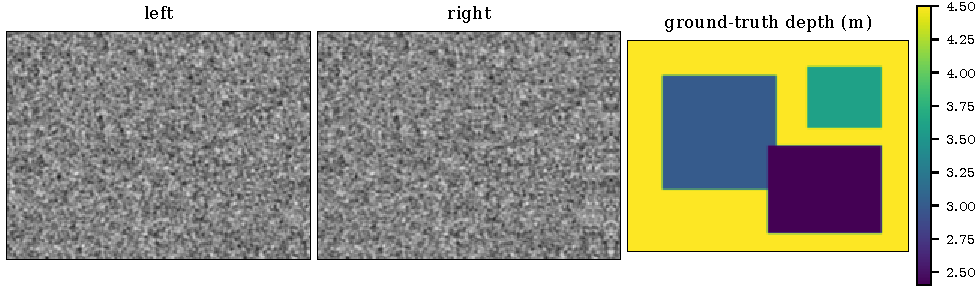
\includegraphics[width=\textwidth]{fixture.pdf}
  \caption{The analytic fixture at seed 0: the stereo pair and the ground-truth
  depth field behind it, at the parameters every analytic-fixture result in this
  report was measured at --- $240\times320$, $f = 700$\,px, baseline 65\,mm.
  Depth is present only in disparity; neither monocular image contains it, which
  is the property Julesz's construction was designed
  for~\cite{julesz1960binocular}. \emph{Regenerated} from
  \texttt{make\_synthetic\_scene(seed=0)}, ported unchanged from
  \texttt{visgraf/bioeye@e908170}~\cite{bioeye}. The figure asserts
  \texttt{gap-010}'s first mechanism before drawing: zero right-image values
  fall outside the left image's range, because the right image is resampled from
  the left rather than rendered.}
  \label{fig:fixture}
\end{figure}

Random-dot stereograms are the right synthetic fixture for this work, for the
reason Julesz introduced them: depth exists only in disparity, so nothing can be
recovered by exploiting shading or texture gradient. The fixture used here
follows the standard construction --- generate a texture, then warp it by the
ground-truth disparity field to produce the second view.

That construction has a defect, and it is not the obvious one.

At a depth discontinuity the disparity field jumps, so adjacent output pixels
draw from widely separated input columns. The second image acquires a stretched
or duplicated patch of real texture with no consistent disparity. The matcher
finds it. The result is a confident, incorrect depth estimate --- and it
survives the front end's validity test, of which left--right consistency is one
of two conditions: 78.5\% of discontinuity pixels are marked valid, and 21.7\%
of those are wrong by more than two pixels.

The obvious criticism of a warped stereogram is that it lacks true
half-occlusions. The measured problem is worse and has the opposite sign: the
fixture substitutes an artefact that is harder than real occlusion and invisible
to the detector meant to catch it. Rendering the same geometry in a
physically-based renderer, where occluded pixels genuinely have no correspondent
and fail consistency, the fixture is 23\texttimes{} worse in the tail at depth
discontinuities and 1.6\texttimes{} worse in the median. The damage is
concentrated in a small number of badly wrong estimates rather than spread
across the field --- which is what an artefact that passes validity looks like.

The pixels within ten of a depth discontinuity are 38\% of the valid measured
pixels and carry 82\% of the total squared error.

\begin{figure}[htbp]
  \centering
  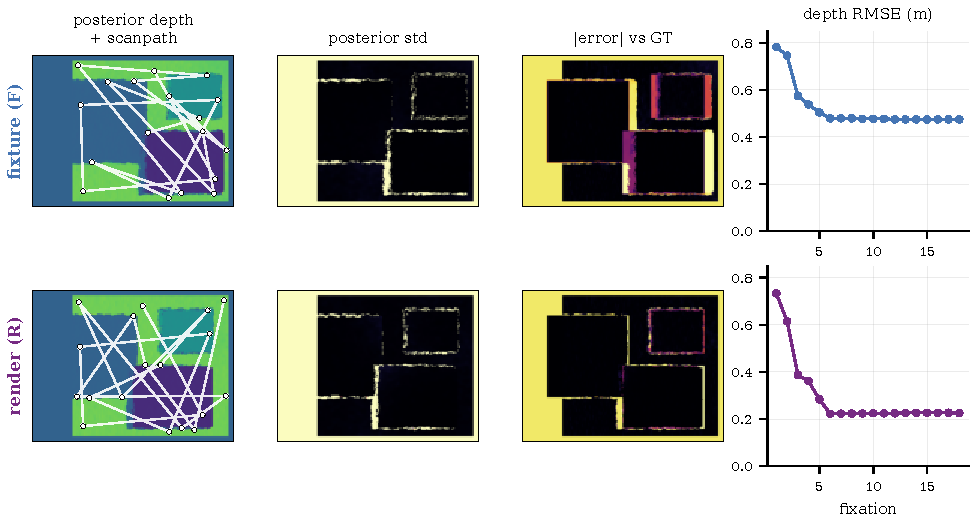
\includegraphics[width=\textwidth]{diagnostic.pdf}
  \caption{The same geometry from two sources, at seed 0, under the ported loop
  with policy \texttt{A'} for 18 fixations: the analytic fixture (F), whose
  right image is resampled from its left, and a Blender render (R), where
  occluded pixels genuinely have no correspondent. The fixture's error
  concentrates in bands at the depth discontinuities that the render's does not
  have, and its RMSE settles at 0.475\,m against the render's 0.225\,m.
  \emph{Measured}: exp004, whose recorded band figures are \texttt{AT} p90
  1.4982\,m for F against 0.0734\,m for R
  (\texttt{experiments/exp004\_scene\_model\_check/results.json}). The panels are
  regenerated from committed code at the pinned seed because exp004 stored no
  arrays; both regenerated scanpaths are asserted against the two the experiment
  recorded before the figure is drawn, and the two loops agree on 1 of 18
  fixations.}
  \label{fig:diagnostic}
\end{figure}

% Set from report/draft.md section 4. The prose is the maintainer's; this file is
% its transit into LaTeX and nothing in it was rewritten.
\section{Findings}

\subsection{Summary}

Thirteen experiments produced a set of results that read at first as unrelated:
some about the synthetic stimulus, some about the gaze policy, one about closing
the loop. They are better understood as one claim measured at three levels.

\begin{quote}
\textbf{Availability dominates selection.} What can be measured determines the
result. How cleverly one chooses among what can be measured is a second-order
refinement. This holds whether the thing limiting availability is the stimulus,
the sensor's field, or the geometry of occlusion.
\end{quote}

Each experiment was designed to answer the question in front of it --- does the
objective matter, does variance help, does verging acquire anything --- and the
pattern across them became legible only once the instrument was characterised
well enough that the answers could be trusted. \S4.2 asks what selection buys;
\S4.3 asks what changes availability.

Two consequences of \S3.3 have to be carried forward, because both were
reversals.

Conclusions already drawn had to be re-read, because results measured on the
fixture were pooled over a pixel population dominated by the artefact.

And the obvious correction was also wrong. Restricting the analysis to pixels
far from any discontinuity made every policy difference vanish, which looked
like a clean answer: the effects had been artefactual. On rendered data they
returned, stronger. Removing discontinuities does not isolate \emph{clean}
measurement --- it isolates \emph{easy} measurement, and on smooth textured
surface there is nothing to allocate. The band where the artefact lived is also
the band where the question lives, which is why the artefact was so damaging and
why removing it by masking answers nothing.

A stimulus, once characterised, also has an operating range. Sweeping the
fraction of occluded surface showed the allocation question is sharpest near a
tenth of the surface occluded --- and, independently, that the acquisition gain
measured later peaks at the same level. Above roughly a sixth the stimulus stops
discriminating between policies altogether, and not merely because the spread
grows: the arms' error means themselves converge, from a spread of 0.51 at a
tenth to 0.02 at a sixth, as the scene's own difficulty saturates the estimator.
That range then sized every experiment after it.

A stimulus is an instrument. Four of thirteen experiments went to establishing
that, and none of the results after them would have been readable otherwise.

\subsection{What selection buys}

The gaze policy proposes a next fixation by maximising something over the
current belief. The natural candidate is posterior variance: look where you are
least certain.

\textbf{The choice of objective does not matter.} Two objectives were compared
--- variance, and the expected reduction in variance a fixation would actually
produce, integrated over the field. They never once selected the same pixel: an
agreement rate of exactly zero across 144 comparisons, and zero again across a
further 144 for a second pairing. Their picks sit a median 115 pixels apart,
more than three fovea widths --- different regions of the image, not
neighbouring cells. And their results were indistinguishable under the
experiment's pre-registered bar, with a sign test agreeing there is no effect.

The fields are moderately rank-correlated, so this is a statement about the
argmax rather than about the objectives being unrelated. It is also a statement
about one fixture, with both objectives evaluated at the same state on the same
candidate grid, so that only the objective varies.

\textbf{What matters is not looking twice.} Posterior variance conflates two
situations: \emph{nothing has been measured here yet}, and \emph{measurement
here is known to be uninformative}. The second is a fixed point --- looking
again does not reduce it. Without a mechanism to suppress recently-visited
locations, the policy locks: in one representative run it visited eight distinct
locations and then spent its remaining ten fixations on a single pixel, where
the matcher had confidently hallucinated a disparity and the confidence
machinery had correctly refused it.

\begin{figure}[htbp]
  \centering
  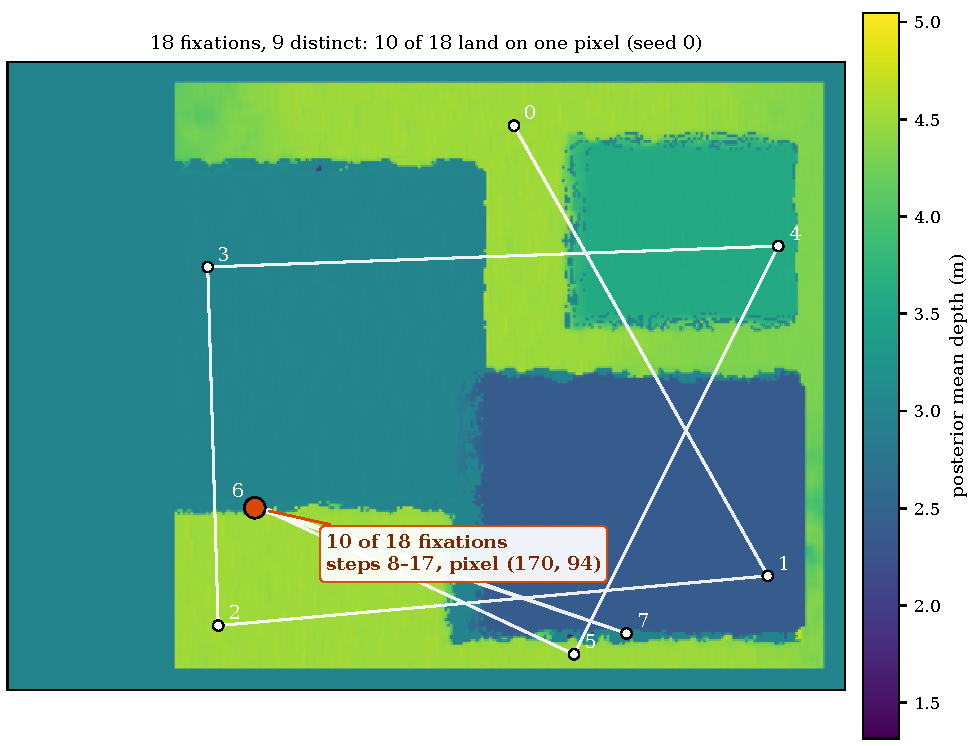
\includegraphics[width=\textwidth]{scanpath.pdf}
  \caption{Scanpath of the ported baseline under argmax-posterior-variance
  selection with no inhibition of return, on the analytic fixture at seed 0.
  Eighteen fixations, nine of them distinct: the loop visits eight pixels once
  each, reaches pixel $(170, 94)$ at step 8, and spends its remaining ten
  fixations there. Step 6 lands at $(169, 94)$, one pixel above the lockup
  pixel, so its marker sits beneath the highlighted one at this scale.
  \emph{Measured}, and regenerated for this figure from committed code at a
  pinned seed: \texttt{bio-001} and \texttt{bio-002} in
  \texttt{docs/inherited-measurements.yaml}, pinned by
  \texttt{tests/test\_loop\_port.py}. This is the predecessor's loop, ported
  bit-identically (\texttt{bio-009}); it is inherited behaviour and a baseline,
  not a result about anything new.}
  \label{fig:scanpath}
\end{figure}

\textbf{Knowing where measurement is possible beats knowing how well.} A policy
informed only by the validity mask --- no variance at all, just \emph{don't look
where nothing can be measured} --- captures the overwhelming majority of the
available benefit. On median error, on a stimulus with effectively no occlusion,
knowing \emph{where} the data is was worth 65\texttimes{} what knowing \emph{how
uncertain} it is added on top. On the tail the ratio narrows to 3.5:1, and it
falls as occlusion rises. Variance is a real refinement, and a second-order one.

That refinement was nearly lost to the instrument. On the fixture, variance
appeared to contribute nothing once the artefact band was excluded. On rendered
data it recovered, several times stronger than the fixture had ever shown. The
fixture was understating the saliency channel, not inflating it --- the opposite
of the concern that prompted the check.

\textbf{Foveal weighting, on a uniformly sampled sensor, is strictly lossy.}
Given a complete spherical capture --- every direction present, nothing outside
the field --- a gaze-dependent foveal weight lost to uniform weighting on both
metrics, in every band grouping, on every one of eight seeds. The mechanism is
measured: the solid angle receiving more than one percent of peak weight is the
whole sphere for uniform weighting and about a fifth of it for foveal, so the
foveal arm leaves four fifths of the sphere at the prior. The reason is
structural rather than empirical --- a foveal weight models an \emph{acuity
gradient}, and a uniformly sampled sensor does not have one. Weighting by gaze
can only discard information already paid for. It cannot buy anything back.

This does not mean allocation is worthless. It means allocation implemented as
weighting, on a sensor with no acuity gradient, has nothing to work with.

\subsection{What changes availability}

If selection buys little, the remaining hypothesis is that active vision works
by changing what is available rather than by choosing among it.

\textbf{Deliberately verging to acquire made things worse.} Narrowing the
disparity search around the current vergence estimate, so that re-verging brings
new depths into range, cost 7.5\texttimes{} in median accuracy. Verging to
re-acquire did not recover it: it halved the tail and bought 21.7\% more
coverage, at 2.6\texttimes{} the hypothesis count and nineteen front-end calls
against one.

The mechanism is the interesting part, and it is not specific to vergence. The
estimator computes a statistic over \emph{valid} measurements in a foveal
window, and a target outside the search range either fails validity or clamps to
the edge --- so the pixels carrying the error are the ones the validity mask has
already deleted. At one measured fixation the target sat at nineteen pixels of
disparity while the estimator's window reported eight, and the controller verged
away from it, from ten pixels to six over three fixations. Across the run it
partially recovers, and it is better described as badly steered than as stuck.
\S5 returns to this as the finding with the widest reach beyond stereo.

\textbf{Closing the perception-action loop does help.} Re-rendering at each new
fixation, re-matching, and accumulating into a head-centred belief beats holding
a single capture and re-weighting it, at 41\texttimes{} the cost in wall-clock
seconds --- of which the renders are 91\%.

It helped at every occlusion level tested, consistently in direction: the moving
arm was better in all sixteen band-by-level cells. It was not consistent in
verdict. Per band the results are level-dependent and non-monotone, and the
effect at depth discontinuities crosses the bar at the lowest and highest
occlusion levels but not at the two between. A consolidation run at three times
the seeds also revised the original margins downward, because the smaller sample
had underestimated the spread. The conclusion survived; its margin did not.

Decomposing the gain is where the result becomes specific. It splits into an
\emph{accuracy} term, on the cells both arms measured, and a \emph{coverage}
term, on the cells only the moving sensor ever reached. Coverage exceeded
accuracy by at least 33\texttimes{} at every level and by 341\texttimes{} at the
highest, in a decomposition that is exact --- the two terms sum to the total at
every level. The closed loop's value is not that it estimates better; it is that
it sees the scene, and the fixed sensor does not.

\begin{figure}[htbp]
  \centering
  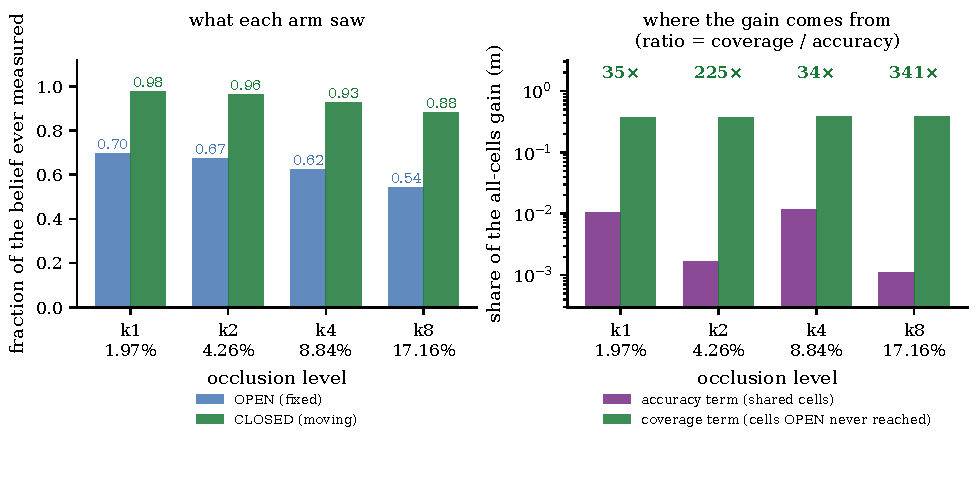
\includegraphics[width=\textwidth]{coverage.pdf}
  \caption{The two arms of exp010/exp011 over four occlusion levels, 24 seeds
  each. \emph{Left}: the fraction of the belief each arm ever measured.
  \emph{Right}: exp011's question-3 decomposition of the all-cells gain into an
  accuracy term, on the cells both arms reached, and a coverage term, on the
  cells only the moving arm reached; note the logarithmic axis. \emph{Measured}:
  exp011, on the pre-registered yardstick of mean absolute error over all
  76\,800 cells with unmeasured cells left at the prior
  (\texttt{experiments/exp011\_consolidation/results.json}, 192 rows;
  \texttt{bio-076}). The decomposition is exact --- the two terms sum to the
  total at every level --- and this figure rebuilds it from the per-seed rows
  and asserts the result against the values exp011 published before drawing.}
  \label{fig:coverage}
\end{figure}

The accuracy term was then narrowed by an experiment whose premise turned out to
be false. Both arms re-estimate vergence at every fixation and both apply the
same foveal weight at the same locations, so they differ in exactly one respect:
whether the images are fresh. Away from depth discontinuities, freezing the
linearisation pedestal costs nothing --- so the advantage there comes from the
fresh captures rather than from re-linearising about each new fixation. At
discontinuities the experiment cannot separate the two, and one confound remains
unexcluded: the stationary arm's measurements are far more correlated with each
other than the moving arm's. The attribution to re-acquisition is established on
smooth surface and open where the geometry is hard.

That is the project's positive result, and it is a narrow one. A second
viewpoint helps. Choosing it cleverly does not.

\textbf{And on a complete spherical sensor, acquisition disappears entirely.}
The eyes rotate about centres fixed in the head; a rotation about a fixed
optical centre does not change what a complete sphere sees. Re-rendering at a
new fixation returns an identical capture. There is nothing to acquire.

\begin{figure}[htbp]
  \centering
  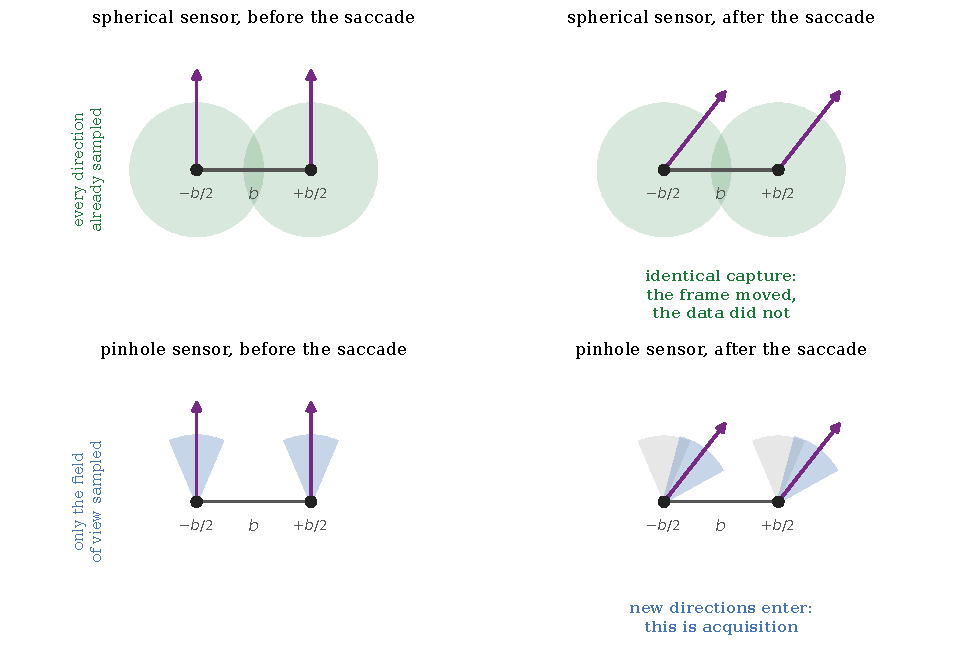
\includegraphics[width=\textwidth]{rig.pdf}
  \caption{Why a saccade acquires nothing on a complete spherical sensor.
  \emph{Top}: two eye centres fixed in the head at $\pm b/2$, each carrying a
  sensor that has already sampled every direction; the gaze rotates and the
  capture is unchanged, because the rotation moves the \emph{frame} and not the
  \emph{data}. \emph{Bottom}, for contrast: on a pinhole sensor the field of
  view rotates with the gaze, and the crescent it uncovers is what acquisition
  means. A conceptual diagram --- it draws a geometric argument, so every
  factual mark traces to a ledger entry, and the script asserts those entries
  exist before drawing. \texttt{fc-013}: the centres are fixed and
  \texttt{eye\_rotations} returns rotations, not translations, so ``a complete
  capture has no hemisphere to hide''. \texttt{bio-081}: a sphere loses no grid
  at any saccade amplitude. \texttt{bio-082}: two orientations, identity and
  yawed $37^\circ$/pitched $19^\circ$, reproduce the same analytic function of
  direction to 80\,\textmu m, measured against a real Blender. \textbf{The
  qualifier is load-bearing}: this holds for a sensor sampled \emph{uniformly}.
  Under variable resolution the fovea resolves what the periphery only sampled
  coarsely, and refixation buys something again (\texttt{od-004}).}
  \label{fig:rig}
\end{figure}

\begin{figure}[htbp]
  \centering
  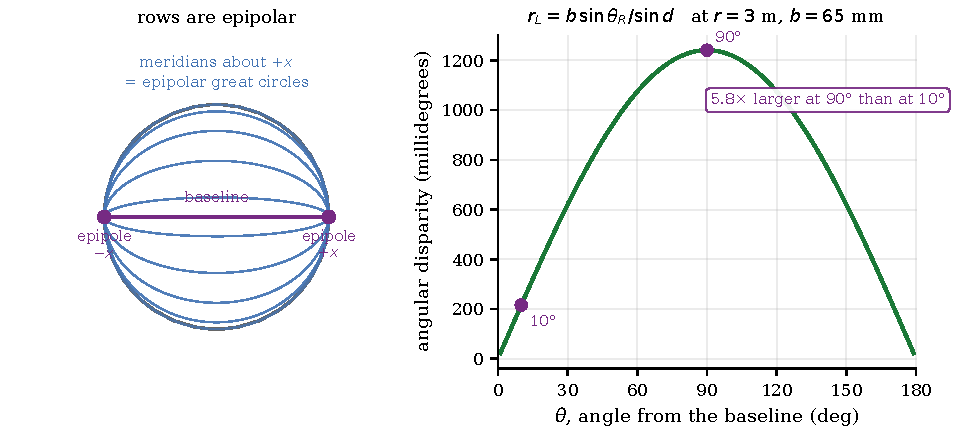
\includegraphics[width=\textwidth]{spherical.pdf}
  \caption{Spherical stereo geometry. \emph{Left}: with the baseline along
  $+x$ the two epipoles sit at $\pm x$, so every epipolar great circle passes
  through them and the family of such circles is exactly the meridians about the
  baseline --- which is why rows of the equirectangular sensor are epipolar and
  the matcher's horizontal shift is a shift in colatitude $\theta$.
  \emph{Right}: the sine rule $r_L = b\,\sin\theta_R/\sin d$ on the triangle
  (left centre, right centre, point) makes the angular disparity depend on
  $\theta$, the angle from the baseline, in a way the pinhole relation $f b / z$
  has no analogue for. \emph{Derived}, closed-form, from the geometry documented
  at \texttt{src/bio3dvision/sampling.py:242--264}, whose stated consequence ---
  at 3\,m the disparity is 5.8\texttimes{} larger at $\theta = 90^\circ$ than at
  $10^\circ$, here 5.76\texttimes{} --- this figure asserts before drawing. The
  relation was checked against a render to $10^{-14}$ relative
  (\texttt{bio-077}).}
  \label{fig:spherical}
\end{figure}

That is not a limitation of the implementation. It is the geometry, and it sets
up the question \S5 takes as its subject.

% Set from report/draft.md section 5. The prose is the maintainer's; this file is
% its transit into LaTeX and nothing in it was rewritten.
\section{Conclusion}

\subsection{Contributions}

\textbf{A structural blindness in control layers driven by masked measurements.}
A controller whose error signal is computed as a statistic over \emph{valid}
measurements cannot see the error that would correct it, because the
measurements carrying that error are the ones validity has already discarded. In
the case measured here, a vergence controller took a robust statistic over valid
disparities in a foveal window; a target outside the search range either failed
the validity test or clamped to the window edge, so the controller had no way to
report \emph{too near} or \emph{too far}. It verged away from its target while
every measurement it could see said it was doing fine.

Nothing about this is specific to vergence, or to stereo. It arises wherever a
validity mask sits upstream of a control loop, which is a common arrangement.
The correction is not a better statistic but a channel that can report \emph{out
of range} --- something the discarded measurements are the only evidence for.

\textbf{Availability dominates selection.} Across the policy experiments, the
binary question \emph{can this be measured at all} outweighed the continuous
question \emph{how well} by 65:1 on median error. Closing the loop helped, and
its benefit was coverage over accuracy by at least 34\texttimes{} at every
occlusion level. Two objectives that never once agreed on a pixel produced
indistinguishable results. The consistent finding is that what limits an active
vision system is what it can see, not how cleverly it chooses among what it can
see.

\textbf{Geometric confinement as a confidence mechanism.} Expanding the depth
relation about the fixated disparity is exact at the fovea and degrades as the
square of the offset. That degradation term inflates the variance of any
estimate far from the fixated depth --- which is to say, precisely the
confidently-wrong matches that anti-calibrated stereo confidence produces. A
term introduced to bound approximation error turns out to function as a filter
against exactly the failure mode the confidence channel cannot report. It is a
property of the estimator, not of the sensor, and it transfers to passive stereo
unchanged.

\textbf{A synthetic stimulus is an instrument and must be characterised before
it is used to measure.} The random-dot fixture used here substituted, at every
depth discontinuity, an artefact both harder than real occlusion and able to
pass the validity test meant to catch it. Four of thirteen experiments went to
establishing this, and every result before them had to be re-read afterwards.

\subsection{What we may have measured}

The negative results are consistent and, taken at face value, they say that
uncertainty-driven active vision does not improve stereo depth estimation. We
are not confident that is the right reading, and the reason is worth stating
precisely.

\textbf{The biological inspiration transferred at the wrong level of
abstraction.} In a retina, foveation means \emph{not paying} for the periphery
--- the samples are never taken. Here it was implemented as \emph{paying, then
discounting}: every pixel matched at full resolution, then weighted down by
distance from gaze. Under that translation a foveal weight can only remove
information already bought, and the measurements show it removing. The mechanism
was not wrong. The level was.

That generalises. If sampling is free, looking is pointless. A complete
spherical capture already contains every direction; rotating the eyes about
their fixed centres returns an identical image, and there is literally nothing
to acquire. Looking matters exactly when sampling is scarce. Every experiment
reported here gave the system unlimited uniform sampling and then asked whether
choosing where to attend helped --- and under that setup the answer nearly has
to be no.

So the honest summary may not be \emph{active vision does not work}. It may be
\textbf{we posed a budget problem as an estimation problem.} The framework's
remaining untested form --- a sensor whose periphery is genuinely sampled more
coarsely than its fovea --- is not one more experiment in the series. It is the
first one that asks the question in the terms the biology poses it.

\subsection{On simulation as an instrument}

A second thread runs through this work and deserves stating on its own.

In simulation-based science the instrument is authored by the same hand as the
hypothesis. The fixture's artefact was not merely a limitation; it was
adversarial to its own detector --- self-consistent enough to pass the validity
test, wrong enough to poison the estimate, and concentrated in exactly the
region where the scientific question lived. Real data can be difficult, biased,
or insufficient. It is not written by someone who wants a particular answer.

We do not think this argues against synthetic stimuli, which offer dense ground
truth no capture provides. It argues that a synthetic stimulus deserves the same
scrutiny as an unfamiliar sensor: characterise its failure modes before trusting
a measurement made through it, and expect its worst behaviour to coincide with
the regime you care about, because that is usually the regime that is hardest to
synthesise.

\subsection{Directions}

\textbf{Variable-resolution sampling} is the priority, for the reason \S5.2
gives --- it is the only formulation in which the question is well posed. It
requires a matcher that operates on a non-uniform lattice, which is a research
problem rather than an engineering one and should be scoped as such. It also
changes the metric: the claim becomes \emph{the same posterior for less
computation}, which needs a declared computational budget that this project
never had to define.

\textbf{A controlled contrast axis at occlusion boundaries} would connect these
results to the confidence failure that motivated them, and settle whether that
failure is a property of real imagery or of high contrast --- which the two
stimulus families measured so far cannot separate.

\textbf{A moving head.} Rotations about fixed centres cannot change what a
complete sensor sees; translations can. Acquisition on an omnidirectional rig
requires the rig to move, which reintroduces a mechanical plant this project set
aside as untested rather than refuted.

\subsection{A note on what remains}

The most reusable output of this work is probably not the code, and not the
single positive result. It is a ledger of foreclosed possibilities, each with
the evidence that closed it and the cost of reopening it: the gaze objective
does not matter, verging to acquire harms and why, foveal weighting on a uniform
sensor is lossy, this stimulus cannot support occlusion claims and here is what
it substitutes instead.

Research whose deliverable is a well-ordered set of eliminated options is
awkward to write up and, we suspect, more reusable than most positive claims.
Someone building an active stereo system now knows several things not to try,
and the reasons --- which is a different and more durable kind of result than a
benchmark number.

\begin{figure}[htbp]
  \centering
  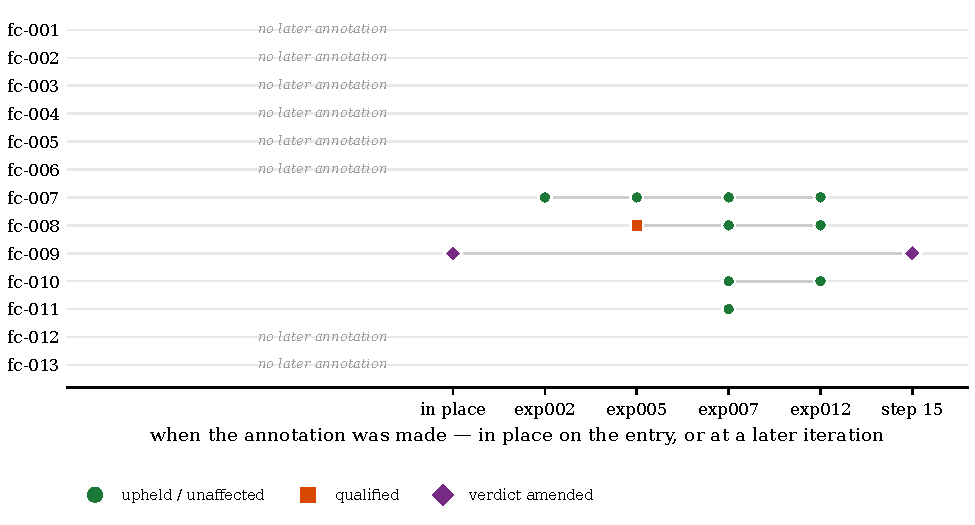
\includegraphics[width=\textwidth]{ledger.pdf}
  \caption{The thirteen foreclosures, and what later work did to each. A
  foreclosure that acquires a qualification acquires it as a new field on its
  own entry rather than as an edit to the original, so the fields are the
  timeline and this figure is built from them rather than from a hand-written
  table. Five of the thirteen were annotated later; eight have not been
  revisited. \texttt{fc-008} is the one that was \emph{qualified} --- by exp005,
  and the qualification did not survive exp007 --- and \texttt{fc-009} is the
  one whose verdict moved twice: written \textsc{additive}, corrected in place
  to \textsc{deferred} because the original overstated what had been measured,
  then answered \textsc{additive} at step 15 once a ray actually crossed the
  boundary. \emph{Derived} from the structure of \texttt{docs/state.yaml}.}
  \label{fig:ledger}
\end{figure}


\section{References}
\printbibliography[heading=none]

\appendix
% Set from report/draft.md, part 4. The prose is the maintainer's; this file is
% its transit into LaTeX and nothing in it was rewritten.
\section{Provenance}

\subsection{How this work was produced}

This project was carried out as a collaboration between one researcher and two
AI surfaces working in different roles. A conversational surface handled
derivation, experiment design, adversarial review, and the specification of each
iteration's work. An agentic coding surface implemented, ran, and verified
against the actual files. The researcher directed the work, took every decision
recorded as a foreclosure, and merged every change.

The division was not decorative. The two surfaces checked each other in both
directions, and both directions produced corrections that reached the record.

Specifications were rejected when their stated assumptions about the repository
turned out to be false --- including one that would have made the sensor unable
to follow gaze in two of its three degrees of freedom, and one whose central
premise about which arms re-estimate vergence was simply wrong. Conversely,
verification against a fresh clone caught claims that had been recorded with
more confidence than their evidence supported.

Every experiment declared, before it was run, what result would falsify the
hypothesis and what result would mean the experiment had asked the wrong
question. Several times the second clause fired. On more than one occasion the
outcome fell outside every direction the falsifier had enumerated, and that
omission is recorded alongside the result.

The corrections are in the record, not smoothed out of it. Where a conclusion
was drawn and later qualified, both the conclusion and the qualification appear,
with the evidence that moved between them. Where a statistical criterion was
inherited from earlier work and used for ten experiments before anyone examined
what it tested, that is recorded too, along with a re-analysis of every affected
verdict.

This report's own prose was verified the same way. Of eighteen substantive
factual claims in the draft, seven stood as written; three were wrong on the
number, and eight were true in the band, arm or metric they came from and
misleading without it. None was unsupported. The verification pass is committed
alongside the report.

We describe the methodology here only as provenance. A separate report treats it
as a subject.

\subsection{Availability}

The repository is public and contains the complete record: every experiment's
pre-registration, runner, raw results, and analysis; the measurement ledger with
each figure's provenance, the commit that produced it, and the environment it
was measured in; the decision ledger with each foreclosure, its evidence, its
stated limits, and the cost of reopening it; and the full commit history, which
was kept forward-only, so corrections appear as amendments rather than as edits.

Figures in this report are generated from that record rather than reproduced
from it.

Measurements carried in from the two predecessor repositories are marked as
inherited --- priors awaiting re-test, not established facts --- and are
distinguished throughout from measurements this project made. Methods carried in
the same way are marked likewise, including the ones never examined.


\end{document}
